\paragraph{The logistic model}
\emph{How should we model the relationship between $\ProbC{X}{Y=1}$ and
$X$?}
\begin{figure}[H]
	\begin{center}
		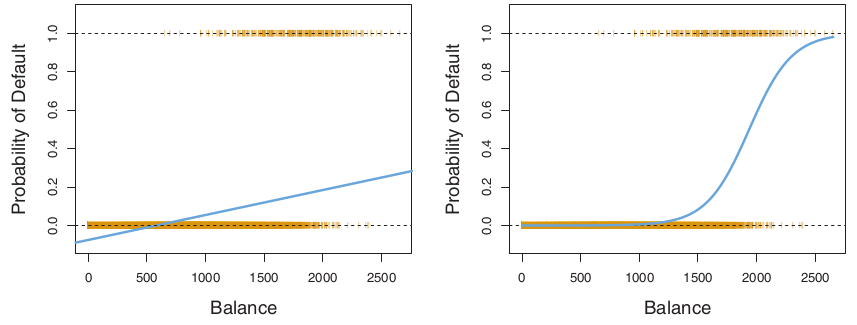
\includegraphics[width=\textwidth]{./chap/1chap/3sec/3images/1ProbabilityOfDefault.png}
	\end{center}
	\caption{Left:Estimated probability of default using linear
regression. Some of estimated probability are negative! The orange 
ticks indicate the $0/1$ values coded for default (NO/YES)\\Right:
Predicted probabilities of default using logistic regression.\\All
probabilities lie between $0$ and $1$.}
	\label{fig:fig3.2}
\end{figure}
\paragraph{The logistic model}
\subparagraph{Assumptions}
\begin{enumerate}
	\item Logistic regerssion must be binary or ordinal.
	\item Mutual independence of observations.
	\item No collinearity
	\item Linearity of qualitative independent variables and log odds.
\end{enumerate}


\subparagraph{Requirement}
\begin{enumerate}
	\item Logistic regression requires quite large sample size.
\end{enumerate}
\subparagraph{Formula}
The logistic regression:
\begin{center}
%	\encN{$p\left(X\right)=\ProbC{X}{Y=1}=\dfrac{e^{\beta_{0}+
%\beta_{1}X}}{1+e^{\beta_{0}+\beta_{1}X}}$}\\
	\encN{$p\left(X\right)=\dfrac{e^{\beta_{0}+
\beta_{1}X}}{1+e^{\beta_{0}+\beta_{1}X}}$}\\
\enc{$\log\left(\dfrac{p\left(X\right)}{1-p\left(X\right)}\right)=
\beta_{0}+\beta_{1}X$}\\ The $\dfrac{p\left(X\right)}{1-p\left(X\right)
}$ quantity is called \emph{odds}.
\end{center}
\paragraph{Estimating the Regression Coefficients}
To fit a logistic model we use the \tR{maximum likelihood} method 
rather that the least squares method (which is a specific case of the
former method). Then we seek estimates $\hb{0}\text{ and }\hb{1}$
such that the predicted probability $\widehat{p}\left(x_{i}\right)$ of
default for each individual corresponds closely as possible to the 
individual default status.
\begin{center}
%	\enc{$\mathcal{L}\left(\hb{0},\hb{1}\right)=\prd{{i:y_{i}=1}}{n}\ProbC{x_{i}}{y_{i}=1}\prd{{j:y_{j}=0}}{n}\left(1-\ProbC{x_{j}}{y_{j}=0}\right)$}\\
\enc{$\mathcal{L}\left(\hb{0},\hb{1}\right)=\prd{i=1}{n}p(x_{i})^{y_{i}}\left(1-p(x_{i})\right)^{1-y_{i}}$}\\
$\hb{0}$ and $\hb{1}$ are chosen to maximize this likelihood function.
\end{center}
%\begin{figure}[H]
%	\begin{center}
%		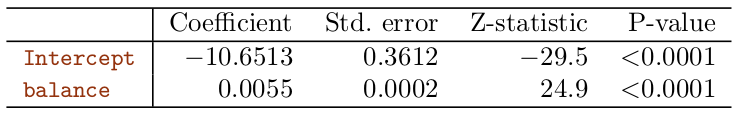
\includegraphics[width=\textwidth]{./chap/1chap/3sec/3images/2estimatesCoeffsLR.png}
%	\end{center}
%	\caption{Estimated coefficients of the logistic regression 
%	model that predict the probability of default using balance.\\
%	A once unit increase in balance is associated with an increase
%	in the log odds of default by $0.0055$ units.}
%	\label{fig:fig3.2}
%\end{figure}
\tB{The \emph{$z$-statistics} plays the same role as \emph{$t$-statistic} in
the linear regression output, $z=\frac{\hb{1}}{SE\left(\hb{1}\right)}$.}
\\The estimated intercept is typically not of interest, its main 
purpose is to adjust the average fitted probabilities to the proportion
of ones in the data.
\paragraph{Marketing Plan}
%\begin{figure}[H]
%	\begin{center}
%		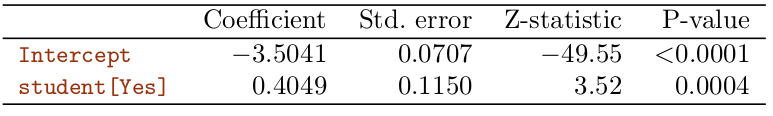
\includegraphics[width=\textwidth]{./chap/1chap/3sec/3images/3LRonDummyVariable.png}
%	\end{center}
%	\caption{Estimated coefficients of the logistic regression
%	model that predicts the probability of default using student
%	status.\\Student status is encoded as a dummy variable, with
%	value 1 for a student and $0$ for a non-student.}
%	\label{fig:fig3.2}
%\end{figure}
$\begin{cases}
	\ProbC{{student=YES}}{\widehat{default}=YES}=\frac{e^{-3.5041+0.4049\times 1}}{1+e^{-3.5041+0.4049\times 1}}=0.0431\\
	\ProbC{{student=NO}}{\widehat{default}=YES}=\frac{e^{-3.5041+0.4049\times 0}}{1+e^{-3.5041+0.4049\times 0}}=0.0292
\end{cases}$\\
This indicates that students tend to have higher default probabilities
than non-student.
\paragraph{Multiple Logistic Regression}
\begin{center}\enc{
$log\left(\dfrac{p\left(X\right)}{1-p\left(X\right)}\right)=\beta_{0}+
\su{{j=1}}{p}\beta_{j}X_{j}$}
\end{center}
%%\begin{figure}[H]
%%	\begin{center}
%%		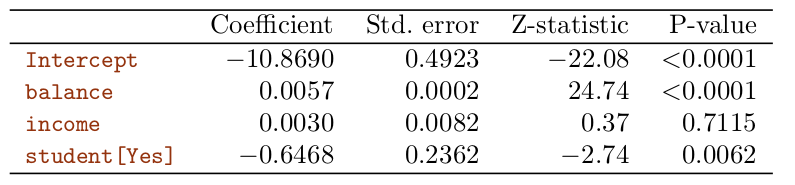
\includegraphics[width=\textwidth]{./chap/1chap/3sec/3images/4multipleLR.png}
%%	\end{center}
%%	\caption{Estimated coefficients of the logistic regression
%%	model that predicts the probability of default using balance,
%%	income and student status.\\Student status is encoded as a
%%	dummy variable, with value 1 for a student and $0$ for a
%%	non-student.\\In fitting this model income was measured in 
%%	thousands dollars.}
%%	\label{fig:fig3.4}
%%\end{figure}
%We surprisingly observe that for given values of income and balance, a
%student is less likely to default than a non-student.
%\begin{figure}[H]
%	\begin{center}
%		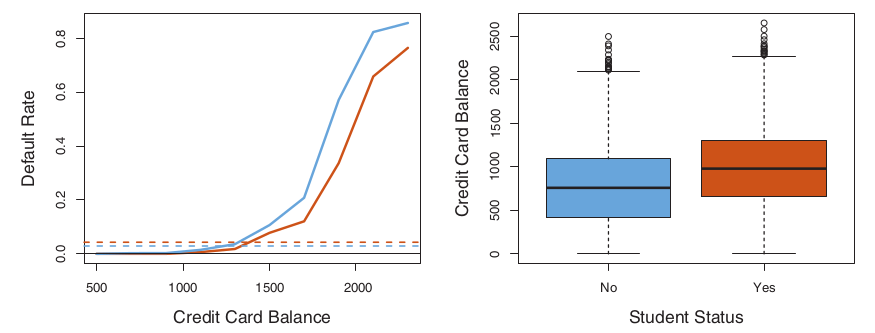
\includegraphics[width=\textwidth]{./chap/1chap/3sec/3images/5confoundingPlot.png}
%	\end{center}
%	\caption{Confounding in the Default data. Left:Default rates
%	are shown for students (orange), and non-students (blue).\\
%	The solid lines show default rate as a function of balance,
%	while horizontal dashed line display the overall default rate
%	\\Right: Boxplots of balance for students and non-students.}
%	\label{fig:fig3.4}
%\end{figure}
%Indeed we observe that from the left-hand panel that the student 
%default rate is at or below of the non-student default rate for every
%value of balance.\\But the horizontal broken lines showing the default
%rate for students and non-students averaged over all values of income
%and balance suggest the opposite effect. Consequently there is a
%positive coefficient for student in the simple logistic regression
%output.\\The right-hand panel provides an explanation for this
%discrepancy, the variables student and balance are correlated. Indeed
%students are more likely to have large credit card balances, which, as
%we know from the left-hand panel tend to be associated to a high 
%default rate. Thus, even though an individual student with a given 
%credit card balance will tend to have a lower probability of default
%than a non-student with the same credit card balance. The fact that 
%students on the whole tend to have a higher credit card balances means
%that overall students tend to default at a higher rate than 
%non-students.
\paragraph{Logistic regression for $p$>2 response classes}
We use \emph{discriminant analysis}
\paragraph{Fitting Logistic Regression Models}
\tB{Logistic regression models are usually fit by maximum of likelihood}, using the conditional 
likelihood of $G$ given $X$. The log-likelihood for $N$ observations is: 
\tB{$$ l(\theta)=\su{{i=1}}{N}log\left( p_{g}(x_{i;\theta}) \right)$$} where $p_{g}(x_{i};\theta)=
\ProbC{X=x_{i}}{G=g;\theta}$.\\
It is convenient to code the two-class $g_{i}$ via a 0/1 response $y_{i}$, where $y_{i}=1$ when
$g_{i}=1$, and $y_{i}=0$ when $g_{2}=2$. Let $p_{1}(x;\theta)=p(x;\theta)$, and 
$p_{2}(x;\theta)=1-p(x;\theta)$. Then the log-likelihood can be written:
\begin{align*}
	l(\beta) =& \su{{i=1}}{N}\left\{ y_{i}\log\left(p(x_{i};\beta)\right)+ (1-y_{i})
	\log\left(1- p(x_{i};\beta)\right)\right\}\\
	=& \su{{i=1}}{N}\left\{ y_{i}\beta^{T}x_{i} - \log\left( 1+e^{\beta^{T}x_{i}} \right) \right\}
\end{align*}

To maximize the log-likelihood, we set its derivatives to zero:
$$ \dfrac{\partial l(\beta)}{\partial\beta} = 
\su{{i=1}}{N}x_{i}\left(y_{i}-p(x_{i};\beta)\right)=0$$ which are $p+1$ equations nonlinear in
$\beta$.
To solve the score, we use the \href{https://en.wikipedia.org/wiki/Newton\%27s_method_in_optimization}{Newton-Raphson} algorithm, which requires the second-derivative or 
Hessian matrix:
$$ \dfrac{\partial^{2}l(\beta)}{\partial\beta\partial\beta^{T}}=\su{{i=1}}{N}
x_{i}x_{i}^{T}p(x_{i};\beta)(1-p(x_{i};\beta))$$
The aim of the Newton-Raphson algorithm is to find the roots of a given real values
function, here $\dfrac{\partial l(\beta)}{\partial\beta}$
Starting with $\beta^{old}$, a single Newton update is : $$ \beta^{new} = \beta^{old} - \left(
\dfrac{\partial^{2}l(\beta)}{\partial\beta\partial\beta^{T}} \right)^{-1}\dfrac{\partial l(\beta)}{
\partial\beta}$$ where the derivatives are evaluated at$\beta^{old}$

Let $\bm{p}$ denote the vector of fitted probabilities with $i^{th}$ element $p(x_{i};\beta^{old})
\text{ and } \bm{W}$ a $N\times N$ diagonal matrix of weights with $i^{th}$ diagonal element
$p(x_{i};\beta^{old})(1-p(x_{i};\beta^{old}))$. Then we have:
\begin{align*}
	\dfrac{\partial l(\beta)}{\partial\beta} =& \bm{X}^{T}(\bm{y}-\bm{p})\\
	\dfrac{\partial^{2} l(\beta)}{\partial\beta\partial\beta^{T}} =&
	-\bm{X}^{T}(\bm{W}-\bm{X})\\
\end{align*}
The Newton step is thus:
\begin{align*}
	\beta^{new} =& \beta^{old} + \left( \bm{X}^{T}\bm{W}\bm{X} \right)^{-1}\bm{X}^{T}(\bm{y}-\bm{p})\\
	=& \left( \bm{X}^{T}\bm{W}\bm{X} \right)^{-1}\bm{X}^{T}\bm{W}\left( \bm{X}\beta^{old}+
	\bm{W}^{-1}(\bm{y}-\bm{p})\right)\\
	=& \left( \bm{X}^{T}\bm{W}\bm{X} \right)^{-1}\bm{X}^{T}\bm{W}\bm{z}
\end{align*}
In the second and third line we have re-expressed the Newton step as a weighted least squares step
with the response: $bm{z} = \bm{X}\beta^{old}+ \bm{W}^{-1}(\bm{y}-\bm{p})$ sometimes known as the
\textbf{adjusted response}.\\
This algorithm is referred to as \textbf{Iteratively Reweighted Least Squares (IRLS)} since each
iteration solves the weighted least squares problem: $$ \beta^{new}\leftarrow\min\limits_{\beta}
\left( \bm{z} - \bm{X}\beta \right)^{T}\bm{W}\left( \bm{z} - \bm{X}\beta \right)$$

It seems that $\beta=0$ is a good starting value for the iterative procedure although convergence
is never guaranteed. Typically the algorithm does converge, since the log-likelihood is concave,
but overshooting can occur.
\tB{Logistic regression models are used mostly as a data analysis and inference tool, where the
goal is to understand the role of the input variables in explaining outcome.}
\emph{Python code}
\begin{python}
import pandas as pd
import sklearn
from sklearn.linear_model import LogisticRegression

y, X = df.iloc[:, 0], df.iloc[:, 1:]
clf = LogisticRegression(random_state=0)
clf.fit(X, y)
print(clf.score(X, y))
\end{python}

\emph{R code}
\begin{rcode}[deletekeywords={model, df, data, family, binomial}]
model.logistic <- glm(y ~ ., data=df, family=binomial)
print(summary(model.logistic))
\end{rcode}
\paragraph{Quadratic Approximations and Inference}
The maximum-likelihood parameter estimates $\hat{\beta}$ satisfy a self-consistency relationship:
they are the coefficients of a weighted least squares fit, where the responses are:
$$ z_{i} = x_{i}^{T}\hat{\beta} + \frac{(y_{i}-\hat{p}_{i})}{\hat{p}_{i}(1_{i}-\hat{p}_{i})}$$

\begin{itemize}
	\item The weighted residual sum-of-squares is the familiar Pearson $\chi^{2}$ statistic:
		$$ \su{{i=1}}{N}\dfrac{(y_{i}-\hat{p}_{i})}{\hat{p}_{i}(1-\hat{p}_{i})}$$ a 
		quadratic approximation of the deviance.
	\item Asymptotic likelihood theory says that if the model is correct, then $\hat{\beta}$
		is consistent.
	\item A central limit theorem then shows that the distribution of $\hat{\beta}
		\hookrightarrow \mathcal{N}\left(\beta,\left(\bm{X}^{T}\bm{W}\bm{X}\right)^{-1} 
		\right)$
	\item Popular shortcuts are the Rao Score test which tests for inclusion of a term, and 
		the Wald test which can be used to test exclusion of a term.
\end{itemize}
